\newpage
\section{INTERRUPTOR PIEZOELECTRICO }
Estos sensores\cite{TE_PiezoFilm} se basan en el efecto piezoeléctrico, donde ciertos materiales generan una carga eléctrica en respuesta a una deformación mecánica. Cuando se aplica una fuerza sobre un material piezoeléctrico, este se deforma y produce una tensión eléctrica proporcional a la magnitud de la fuerza aplicada. Los interruptores piezoeléctricos aprovechan este fenómeno para detectar cambios de presión o vibraciones, generando señales eléctricas que pueden utilizarse para activar o controlar otros dispositivos electrónicos. Son especialmente útiles en aplicaciones que requieren una respuesta rápida y alta sensibilidad, como en sensores táctiles y sistemas de monitoreo de vibraciones.
Estos sensores son fundamentales en aplicaciones de ingeniería electrónica y robótica, permitiendo la medición precisa de fuerzas y la detección de campos magnéticos, lo que es esencial para el control y monitoreo de sistemas mecánicos y electrónicos.\autoref{fig:PIEZO}
\begin{figure}[h]
	\centering
	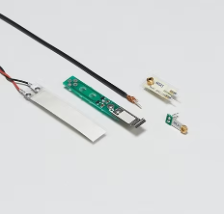
\includegraphics[width=0.3\linewidth]{img/PIEZO}
	\caption{Interruptor piezoecletrico  }
	\label{fig:PIEZO}
\end{figure}

\section{SENSORES EXTERNOS}
\section*{Tipo de contacto}
\section*{Interruptores de límite }
¿Qué es un sensor de contacto?
Los sensores de contacto\cite{Keyence_Contacto} son un tipo de sensor que detecta el final de recorrido de un componente mecánico, es decir, detecta la posición límite de este mismo.\cite{Cybermatics_Sensores} 
\begin{itemize}
	\item  Tipos de sensores de contacto.
	\item  Verticales 
	\item Horizontales 
	\item Micro
\end{itemize}

\begin{figure}[h]
	\centering
	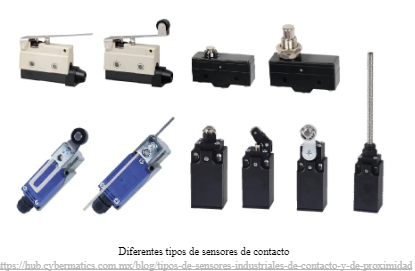
\includegraphics[width=0.3\linewidth]{img/CONTACTO}
	\caption{Sensores de contacto  }
	\label{fig:CONTACTO}
\end{figure}


